\chapter{Plan de test}

Les tests sont essentiels au bon fonctionnement du produit final. Ils permettent de s'assurer que le système est fonctionnel,
respecte les exigences et ne contient pas de surprises.
Planifier les tests permet d'accélérer et de structurer cette étape laborieuse du projet, en identifiant les objectifs et les priorités des différents tests.
Chaque fonctionnalité doit être testé et documenté correctement. Le plan de tests permet donc de mettre en évidence les tests à effectuer pour chaque fonctionnalité et sous-fonctionnalités,
en identifiant les paramètres à tester, la méthodologie a suivre et les équipements nécéssaires.

\begin{figure}
  \centering
  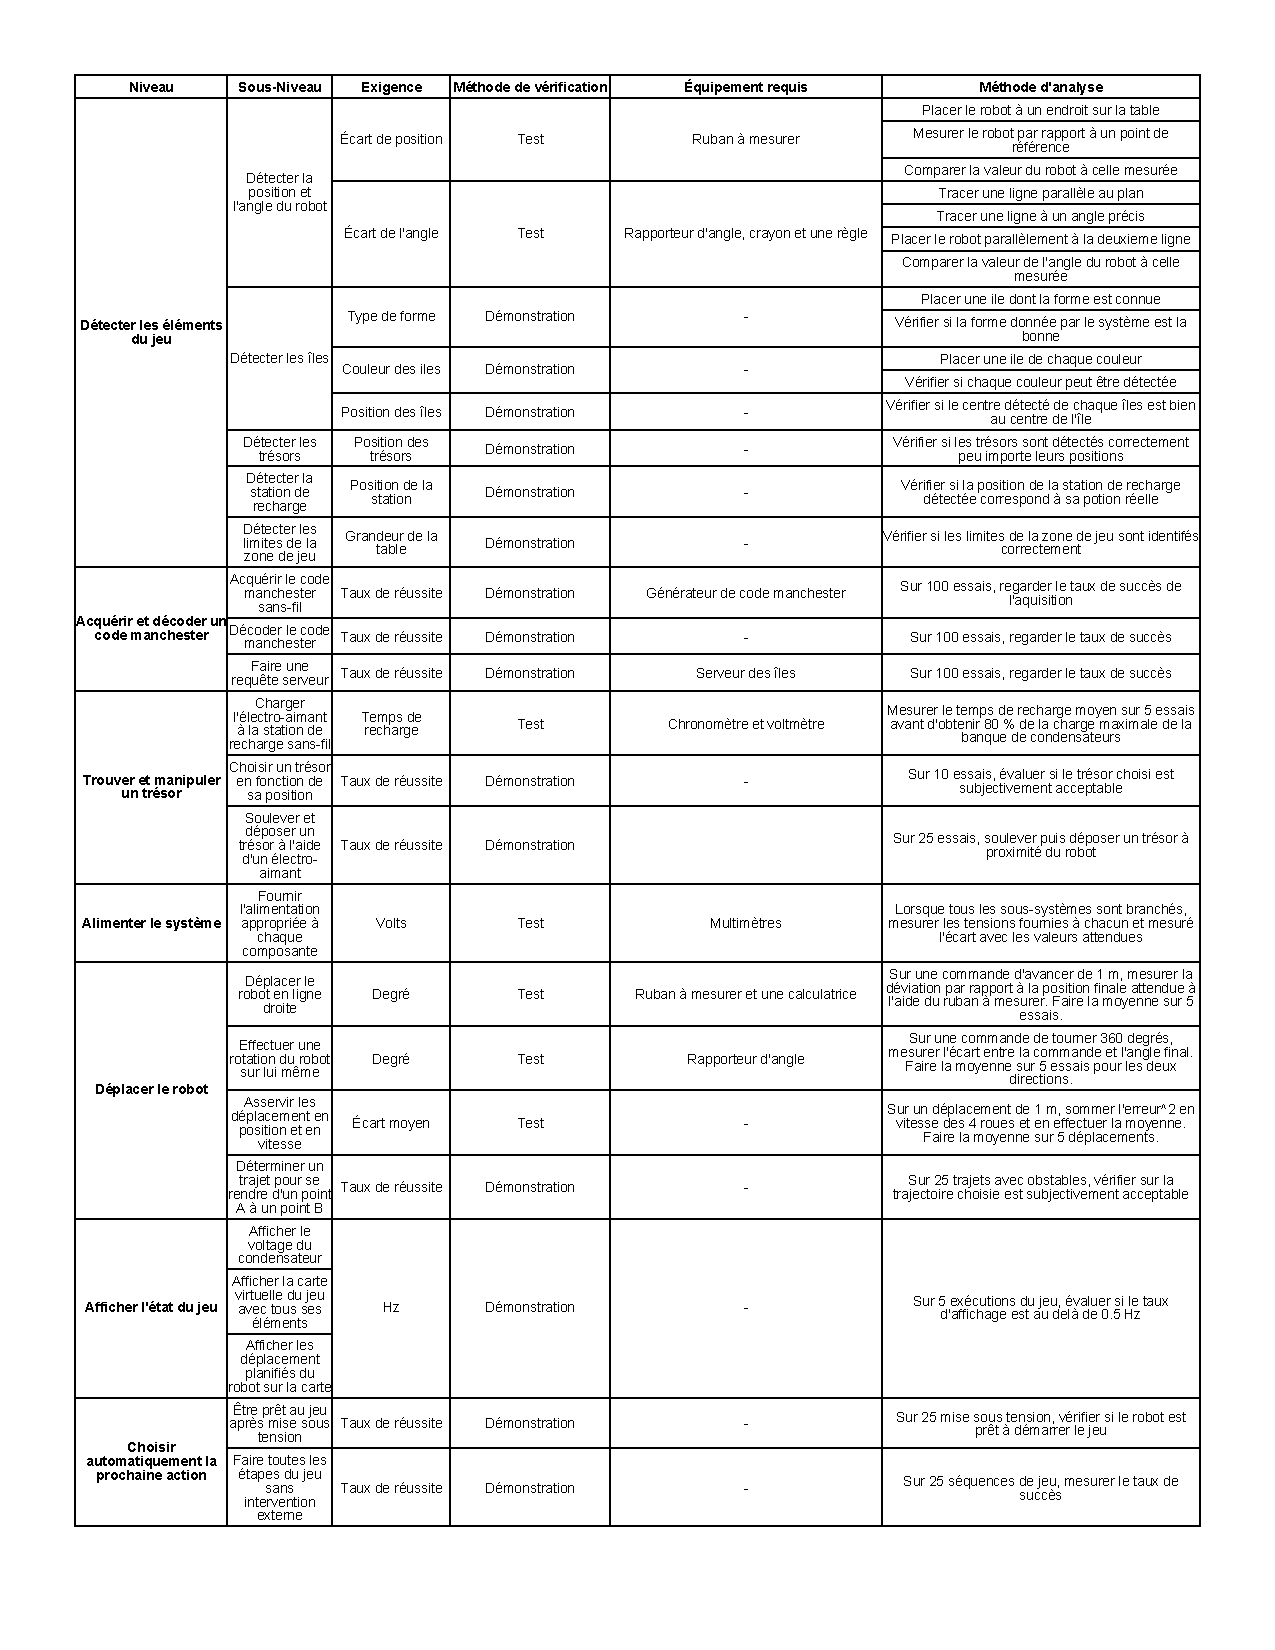
\includegraphics[scale=0.75, angle=0]{resources/tests.pdf}
  \caption{Plan de test}
\end{figure}
